% Figure 3: BanditRouter Architecture Diagram (System Design)

\begin{figure}[t]
    \centering
    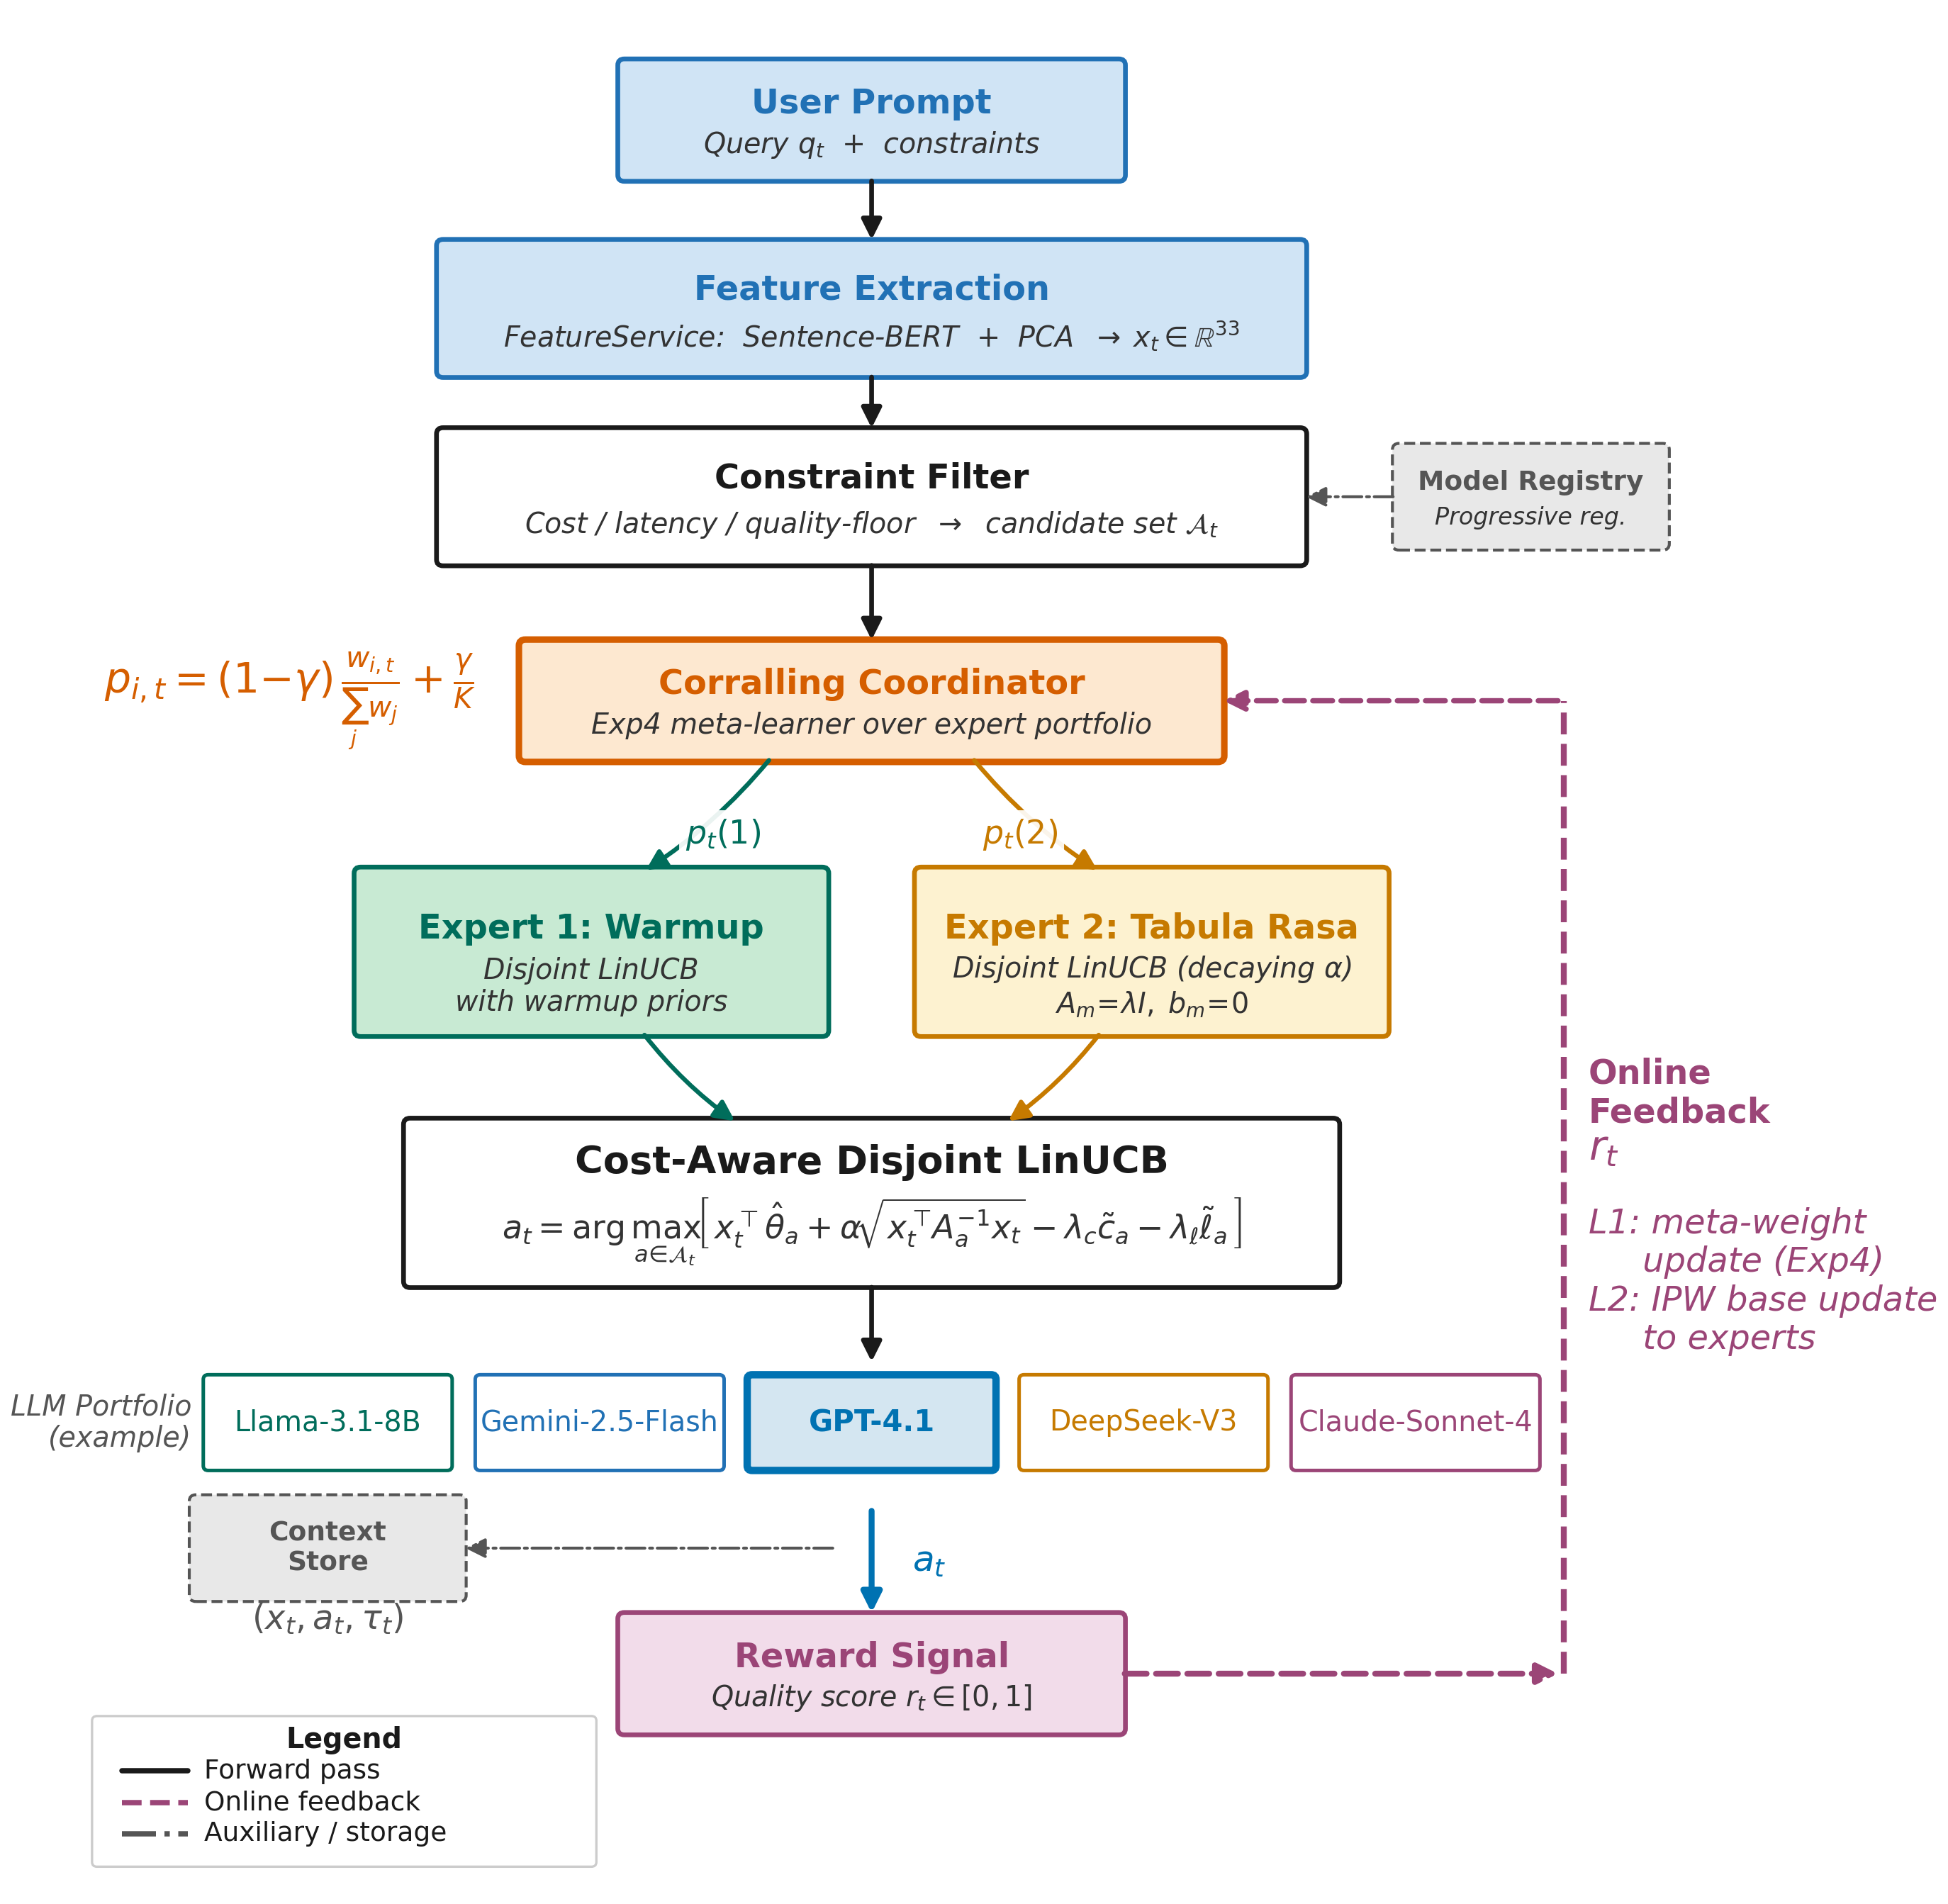
\includegraphics[width=0.85\textwidth]{experiments/02_figure/results/figure2_architecture.pdf}
    \caption{%
        \textbf{Architecture: BanditRouter with Corralling Meta-Learner.}
        The production \texttt{BanditRouter} orchestrates feature extraction,
        constraint filtering, and model selection.
        When multiple model families are present, it activates Hybrid LinUCB
        with family-based parameter sharing.
        The Corralling layer manages two experts via Exp4 meta-learning
        ($\eta{=}\sqrt{\ln K/T}$, $\gamma{=}0.05$):
        Expert~1 (Warmup) initialises with semantic priors and uses constant
        $\alpha{=}2.0$; Expert~2 (Tabula Rasa) learns from scratch with
        decaying $\alpha{=}1.0 \to 0.01$.
        At each request, \texttt{route()} samples an expert with
        probability $P_t = (1{-}\gamma)\,w_t + \gamma/K$ and
        \texttt{process\_feedback()} updates weights via importance-weighted
        loss $\hat{\ell}_t = (1{-}r_t)/P_t$.
        Figure~\ref{fig:prior_degradation} shows that Corralling outperforms
        tabula rasa at good prior quality ($\alpha \leq 0.2$), with a
        crossover at $\alpha \approx 0.3$.
    }
    \label{fig:corralled_architecture}
\end{figure}
